[96~v\textsuperscript{o}] Notandum ⟨27.⟩ illos pollices semper nihil agere (in aere clauso) residuum  agit in funiculum\protect\index{Sachverzeichnis}{funiculus}. Hinc si non satis forte sit suspensum manebit  ut si non sit aequale ipsi Tubo implendo. Hinc si aeris Elaterium\protect\index{Sachverzeichnis}{elaterium}  in summa deminuatur descendet. Hinc sequitur caetera omnia  ab aeris difformitate, hoc experimentum vero Torricellianum\protect\index{Sachverzeichnis}{experimentum!Torricellianum} ab  ejus pondere oriri. Ecce ergo duo principia: aeris repugnantiam  ad occupationem loci minoris, et aeris repugnantiam  ad difformitatem. Ab illo Experimentum Torricellianum\protect\index{Sachverzeichnis}{experimentum!Torricellianum}, ab hoc caetera omnia.  Nota aeris repugnantia ad difformitatem aequalis est  tum in exhausto tum in distento. In aere aperto \edtext{coincidunt, repugnantia aeris}{\lemma{coincidunt,}\Afootnote{ \textit{ (1) }\ gravitas\protect\index{Sachverzeichnis}{gravitas|textit} \textit{ (2) }\ repugnantia aeris \textit{ L}}} ad difformitatem et \edtext{repugnantia ejus ad elevationem vel compressionem}{\lemma{et}\Afootnote{ \textit{ (1) }\ compressionem \textit{ (2) }\ aeris pressio\protect\index{Sachverzeichnis}{pressio!aeris|textit} \textit{ (3) }\ repugnantia [...] compressionem \textit{ L}}},  totus enim tunc aer una massa\protect\index{Sachverzeichnis}{massa}; et omnis in eo mutatio talis causat  difformitatem. Et ut res adhuc magis appareat ecce experimentum novum. Mercurius\protect\index{Sachverzeichnis}{mercurius} in Tubo Torricelliano\protect\index{Sachverzeichnis}{Tubus!Torricellianus} delapsus sit ad  altitudinem determinatam, introducatur in eundem in summo  alius Mercurius\protect\index{Sachverzeichnis}{mercurius}, is pendebit vel ex summitate vel in Tubo  libero spatio medio relicto inter ipsum et Mercurium\protect\index{Sachverzeichnis}{mercurius}  Torricellianum. Et cum hic Mercurius\protect\index{Sachverzeichnis}{mercurius!purgatus} \edtext{etiam aere non purgatus}{\lemma{}\Afootnote{etiam aere non purgatus \textit{ erg.} \textit{ L}}} libere suspendatur  in aere cujus pressio nulla est, qui scilicet est ipsemet  dilatatus \edtext{patet hic}{\lemma{dilatatus}\Afootnote{ \textit{ (1) }\ , et contra \textit{ (2) }\ patet hic \textit{ L}}} nullam aliam rationem fingi  posse, quam repugnantiam aeris ad difformitatem  et mensurari potest quanta sit haec repugnantia, quae eadem  est in aere ordinario, et summe rarefacto, et summe  compresso, ut experientia demonstrari potest. Experimentum  hoc erit elegans, \edtext{tantundem descendere  pondus}{\lemma{elegans,}\Afootnote{ \textit{ (1) }\ aerem \textit{ (2) }\ tantundem descendere  pondus \textit{ L}}} in Tubo summe compresso, et summe rarefacto si  tubus ejusmodi potest praelongus, poterunt diversi Mercurii\protect\index{Sachverzeichnis}{mercurius}  per intervalla in eo suspendi, quo nihil est admirabilius. \edtext{An}{\lemma{admirabilius.}\Afootnote{ \textit{ (1) }\ Item in \textit{ (2) }\ An \textit{ L}}} aere libero quoque suspensio ob difformitatem a gravitate\protect\index{Sachverzeichnis}{gravitas} diversa? Ita: cum Tubus scilicet Mercurio\protect\index{Sachverzeichnis}{mercurius} non  impletus. Ergo nec NB in aere libero coincidunt gravitas\protect\index{Sachverzeichnis}{gravitas} massae\protect\index{Sachverzeichnis}{massa} aereae \edtext{aut in aere clauso ab ea orta compressio}{\lemma{aut [...] compressio}\Afootnote{\textit{ erg.} \textit{ L}}} et aeris repugnantia ad difformitatem.  Etsi gravitas massae aereae\protect\index{Sachverzeichnis}{gravitas!aeris} sit a repugnantia Mundi\protect\index{Sachverzeichnis}{mundus}  generali ad disproportionalitatem, orta a circulatione universali\protect\index{Sachverzeichnis}{circulatio!universalis}. Circa Antliam\protect\index{Sachverzeichnis}{antlia} haec experimenta instituenda, primum Antlia\protect\index{Sachverzeichnis}{antlia}  levetur Mercurius\protect\index{Sachverzeichnis}{mercurius}, quod fateor fieri necessario quamdiu ponderis aeris\protect\index{Sachverzeichnis}{pondus!aeris}, mercurio\protect\index{Sachverzeichnis}{mercurius} praeponderat, necesse est enim alterutrum  levari \edtext{}{\lemma{}\Afootnote{levari  \textbar\ (comprimique,) \textit{ gestr.}\ \textbar\ Mercurium \textit{ L}}}Mercurium\protect\index{Sachverzeichnis}{mercurius} aut aeris \edtext{massam\protect\index{Sachverzeichnis}{massa}. Ergo}{\lemma{massam.}\Afootnote{ \textit{ (1) }\ At ubi  plus \textit{ (2) }\ Ergo \textit{ L}}} infallibiliter levabitur antlia\protect\index{Sachverzeichnis}{antlia} \edtext{Mercurius\protect\index{Sachverzeichnis}{mercurius}  usque ad}{\lemma{Mercurius}\Afootnote{ \textit{ (1) }\ ultra \textit{ (2) }\  usque ad \textit{ L}}} 27. pollices, seu ad altitudinem quam habet  in Tubo \edtext{Torricelliano\protect\index{Sachverzeichnis}{Tubus!Torricellianus}. Ubi vero Mercurius elevatus}{\lemma{Torricelliano.}\Afootnote{ \textit{ (1) }\ Ajo vero et ultra levatum iri \textit{ (2) }\  Ubi vero Mercurius elevatus \textit{ L}}} massae\protect\index{Sachverzeichnis}{massa} aeris aequiponderat, jam  ob eam causam elevari amplius non poterit; necesse erit  ergo, continuatis viribus attrahentis si non ultra elevatur Mercurius\protect\index{Sachverzeichnis}{mercurius}, embolum\protect\index{Sachverzeichnis}{embolus} ab eo divelli, ac proinde esse quod  spatium intermedium impleat, ergo vel aerem intrare, aut  si inest distendi, aut si nec intrare possit nec insit ex Mercurio\protect\index{Sachverzeichnis}{mercurius} subjecto produci, aut ex ipso Mercurio\protect\index{Sachverzeichnis}{mercurius}  subjecto substantiam quandam tendibilem elici necesse  \edtext{est. Nota si Mercurius}{\lemma{est.}\Afootnote{ \textit{ (1) }\ Nam et hoc rationis est ipsum Mercuri \textit{ (2) }\   Nota si Mercurius \textit{ L}}} 
non elevatur ad consuetam altitudinem, necesse est ipsummet aut aerem interjectum  ejus pondere fuisse tensum, quod si aere purgatus est, necesse  erit tendi ipsummet. Cujus rei experimentum capi potest, si  plus quam ante spatii occupat, si scilicet in antlia\protect\index{Sachverzeichnis}{antlia} pendulus est, aut si subjecto in vase  stagnans, videndum an aere hinc  admisso et ab altera parte ob  obstaculum descensu negato,  contrahat sese. Ponamus  vero quicquid ejus sit  separari tandem Embolum\protect\index{Sachverzeichnis}{embolus} a Mercurio\protect\index{Sachverzeichnis}{mercurius}, ob substantiam tendibilem interjectam,  poterit aliquando trahi antlia\protect\index{Sachverzeichnis}{antlia}, sine elevatione Mercurii\protect\index{Sachverzeichnis}{mercurius}, aut cum minore ejus elevatione quam  est ipsius antliae\protect\index{Sachverzeichnis}{antlia}.                      At non in infinitum, ubi  primum enim materia\protect\index{Sachverzeichnis}{materia}  illa eousque tensa  fuerit ut ejus a repugnantia ad tendibilitatem ulteriorem \edtext{gravitatem\protect\index{Sachverzeichnis}{gravitas} liquoris vincat}{\lemma{gravitatem}\Afootnote{ \textit{ (1) }\ aquae vincat \textit{ (2) }\ liquoris vincat \textit{ L}}}, liquor (ultra altitudinem a  contrapondio aeris determinatam) elevabitur  donec tantum ejus elevetur, ut rursus \edtext{tendibilitati}{\lemma{rursus}\Afootnote{ \textit{ (1) }\ contrapondios  liquori \textit{ (2) }\ tendibilitati \textit{ L}}} sit praeponderaturus, sed credibilius  est, elevationem continuam sed pro tendibilitate  deminutam iri. Quod si relinquatur aer  sensibilis intra Embolum\protect\index{Sachverzeichnis}{embolus} et Liquorem, liquor tardius  ascendet quam embolus\protect\index{Sachverzeichnis}{embolus}, ob aeris tendibilitatem  non ergo ob solum massae\protect\index{Sachverzeichnis}{massa} aereae pondus, alioqui tam  cito quam embolus.\pend
% \begin{wrapfigure}{l}{0.2\textwidth}      
%\begin{center}              
%                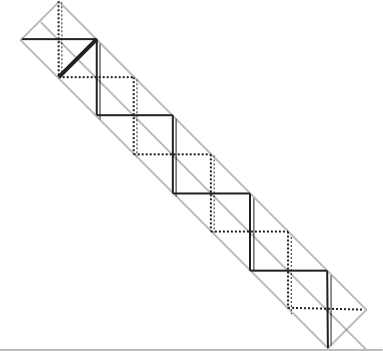
\includegraphics[width=0.5\textwidth]{images/37_3_96v2}\\\textit{[Fig. 9]}
%                       \end{center}
%                        %\caption{Bildbeschreibung}
%                 %      \end{wrapfigure}
%                        %@ @ @ Dies ist eine Abstandszeile - fuer den Fall, dass mehrere figures hintereinander kommen, ohne dass dazwischen laengerer Text steht. Dies kann zu einer Fahlermeldung fuehren. @ @ @ \\
 \pstart  Instrumentum inclinationum\protect\index{Sachverzeichnis}{instrumentum!inclinationum} quo determinari potest  quanta sit vis  ponderis in plano  \edtext{inclinato, quantaque}{\lemma{inclinato,}\Afootnote{ \textit{ (1) }\ \textso{sine} \textit{ (2) }\ quantaque \textit{ L}}} ipsa inclinatio  si in Tubo utrinque clauso Mercurius\protect\index{Sachverzeichnis}{mercurius} sit pendulus  observeturque quousque \edtext{ascendat}{\lemma{quousque}\Afootnote{ \textit{ (1) }\ perveniat \textit{ (2) }\ ascendat \textit{ L}\protect\rule[0cm]{5cm}{0cm}}} Horizontalis, quousque  perpendicularis descendat, spatium hoc dividetur in partes  quot volemus, hae partes, vim dabunt.\pend 
% \begin{center}               
%                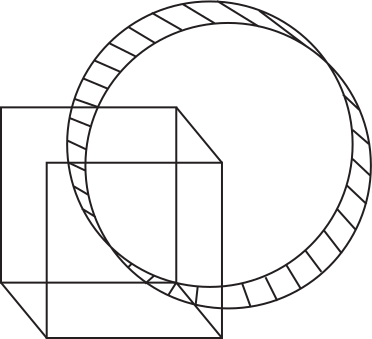
\includegraphics[width=0.4\textwidth]{images/37_3_91v}\\\textit{[Fig. 10 nicht zum Text gehörig]}
%                        %\caption{Bildbeschreibung}
%                        \end{center}
%                     %\pstart\selectlanguage{latin}